\begin{figure}[!htbp]
\centering
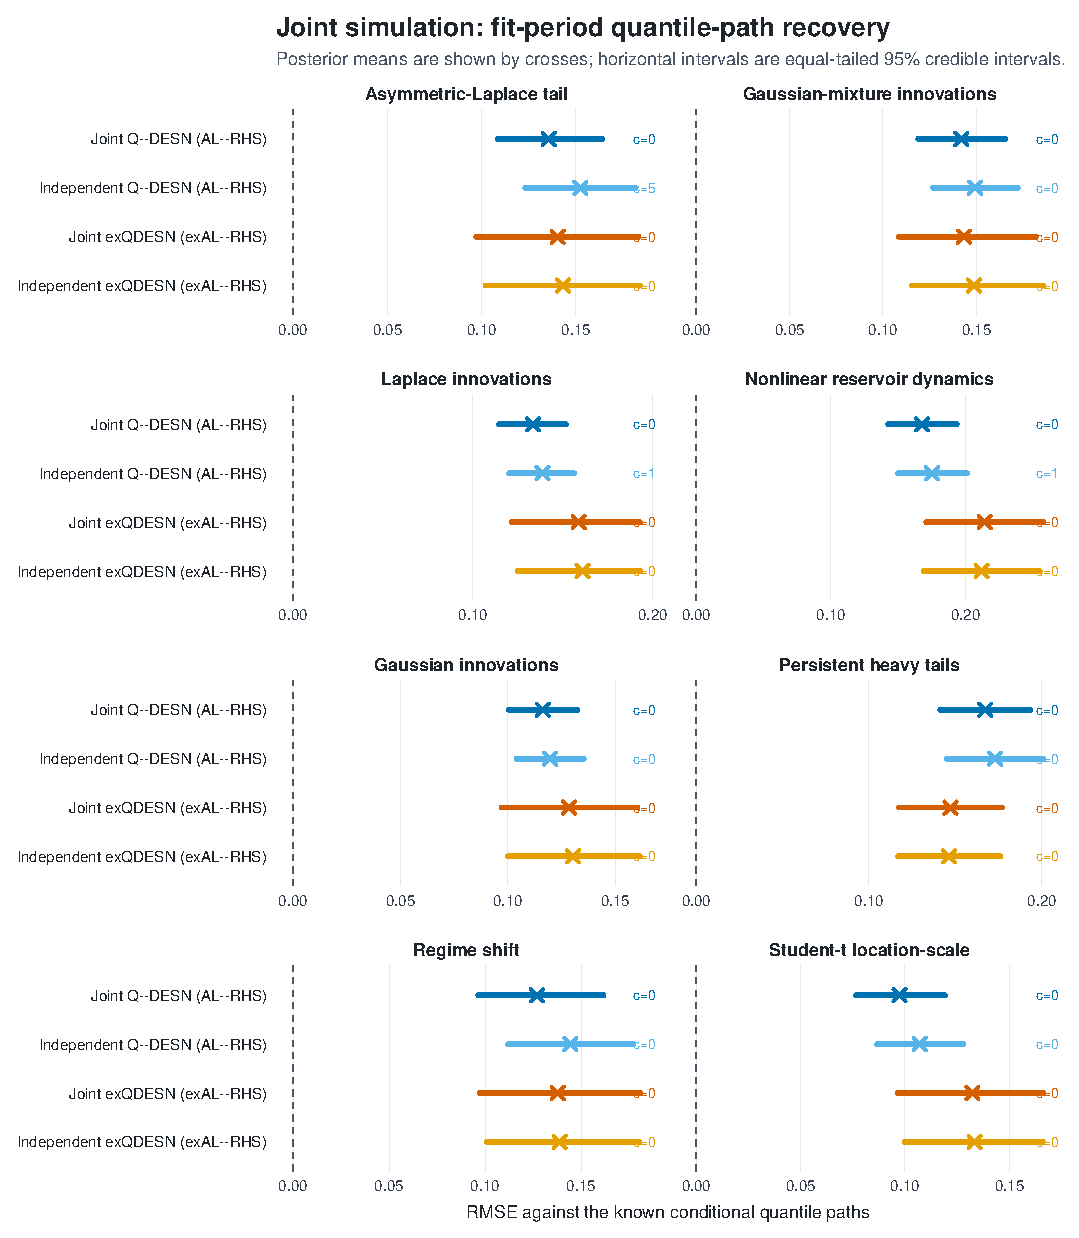
\includegraphics[width=0.98\textwidth]{figures/joint_qdesn_simulation/joint_qdesn_phase181_fit_oracle_rmse_intervals.pdf}
\caption{Posterior fit-period recovery of the known conditional quantile paths in the joint multi-quantile simulation. Each panel uses the same four model classes and the same seven quantile levels. Crosses show posterior means and horizontal bars show equal-tailed 95\% credible intervals computed from 8,000 retained MCMC draws per comparison after monotone rearrangement. Lower RMSE is better. The labels at the right of each panel report raw adjacent-level crossing counts in the posterior-mean fitted grid before monotone rearrangement; all corresponding counts after rearrangement are zero. Panel-specific x-scales are used for readability.}
\label{fig:joint-qdesn-phase181-fit-rmse-intervals}
\end{figure}

\begin{figure}[!htbp]
\centering
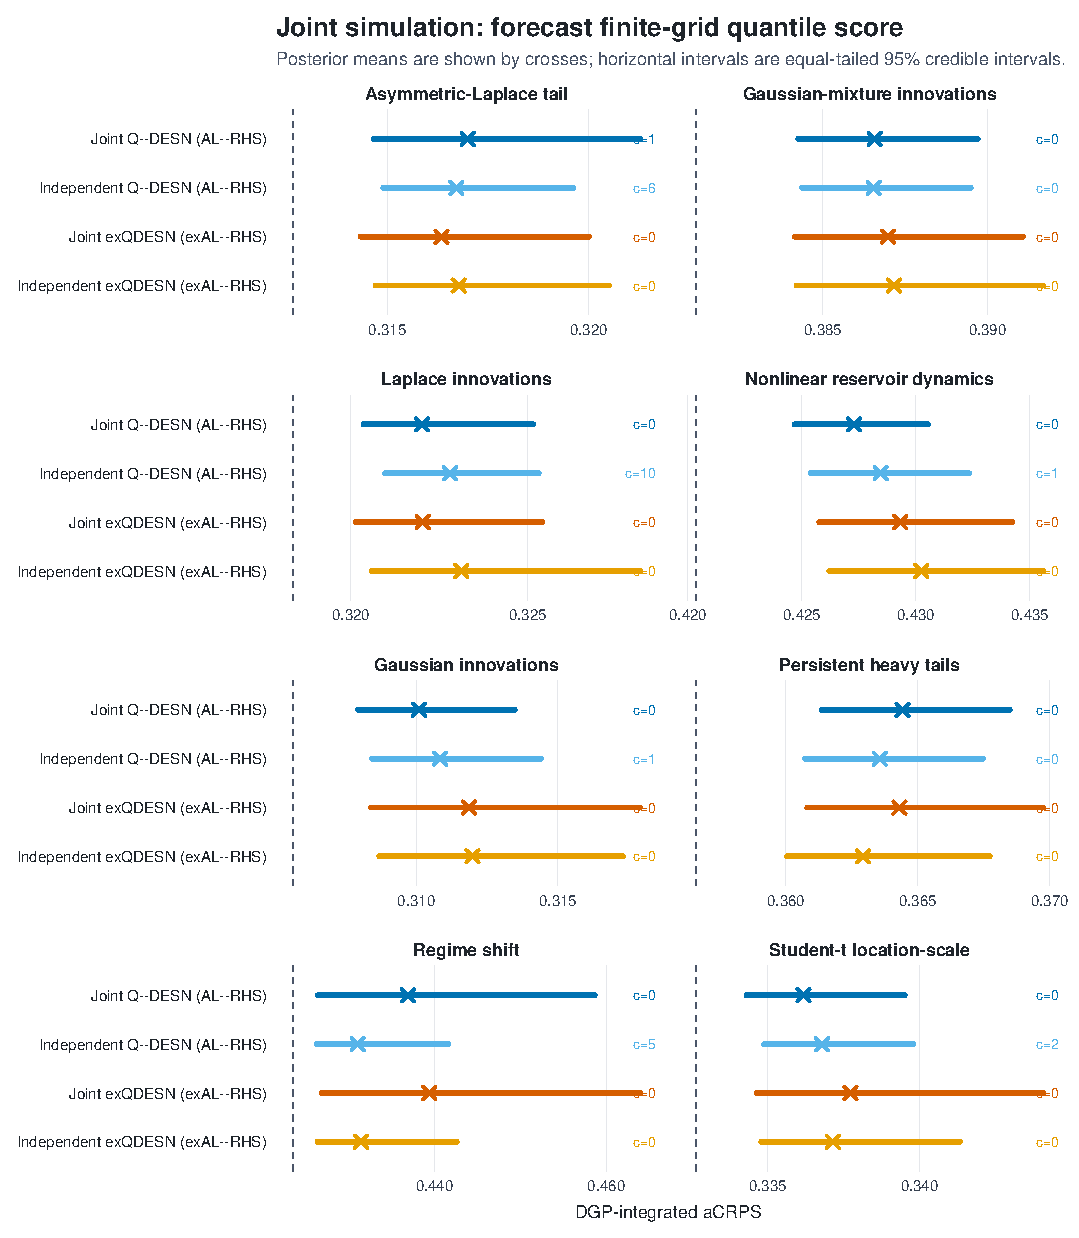
\includegraphics[width=0.98\textwidth]{figures/joint_qdesn_simulation/joint_qdesn_phase181_forecast_dgp_score_intervals.pdf}
\caption{Posterior DGP-integrated finite-grid quantile scores for the joint multi-quantile simulation. Each panel uses the same four model classes, the same held-out forecast design, and the same seven evaluation levels as Table~\ref{tab:joint-qdesn-dgp-integrated-score}. Crosses show posterior means and horizontal bars show equal-tailed 95\% credible intervals from 8,000 retained MCMC draws per comparison. Lower \(\aCRPS\) is better. Dashed vertical lines mark the oracle finite-grid score in each simulation setting. The labels at the right of each panel report raw adjacent-level crossing counts in the posterior-mean forecast grid before monotone rearrangement; all corresponding counts after rearrangement are zero. The numerical rankings remain descriptive because all paired joint-minus-independent contrast intervals include zero. Panel-specific x-scales are used for readability.}
\label{fig:joint-qdesn-phase181-forecast-acrps-intervals}
\end{figure}
